\documentclass[aspectratio=169]{beamer}

% Theme and color scheme
\usetheme{metropolis}
\usecolortheme{default}
\setbeamertemplate{navigation symbols}{}

% Packages
\usepackage[utf8]{inputenc}
\usepackage{amsmath,amssymb,amsfonts}
\usepackage{pifont} % for checkmarks
\usepackage{graphicx}
\usepackage{booktabs}
\usepackage{array}
\usepackage{xcolor}
\usepackage{tikz}
\usepackage{pgfplots}
\pgfplotsset{compat=1.9}

% Custom colors for consistency
\definecolor{ifacblue}{RGB}{0,82,147}
\definecolor{ifacgray}{RGB}{128,128,128}
\definecolor{successgreen}{RGB}{46,125,50}
\definecolor{warningorange}{RGB}{255,152,0}
\definecolor{errorred}{RGB}{211,47,47}

% Set primary color
\setbeamercolor{frametitle}{bg=ifacblue,fg=white}
\setbeamercolor{progress bar}{fg=ifacblue}

% Title page information
\title{Robust Algebraic Parameter Estimation via Gaussian Process Regression}
\author{Oren Bassik\inst{1} \and Alexander Demin\inst{2} \and Alexey Ovchinnikov\inst{1,3}}
\institute{
  \inst{1}CUNY Graduate Center \\
  \inst{2}HSE University \\  
  \inst{3}CUNY Queens College
}
\date{IFAC/COSY/SSSC Joint Conference \\ \today}

% Footer with acknowledgments
\setbeamertemplate{footline}{%
  \begin{beamercolorbox}[wd=\paperwidth,ht=2.5ex,dp=1ex,center]{author in head/foot}%
    \tiny Supported by NSF grants CCF-2212460 and DMS-1853650
  \end{beamercolorbox}%
}

\begin{document}

% Slide 1: Title
\begin{frame}
  \titlepage
\end{frame}

% Slide 2: Intro & Motivation
\begin{frame}[shrink]{Parameter Estimation for ODE Systems}
    \begin{columns}[T]
        \begin{column}{0.48\textwidth}
            \begin{block}{Nonlinear Optimization Methods}
                \small
                E.g., Levenberg-Marquardt, Gradient Descent
                \begin{itemize}
                    \item \textbf{Pros:} Mature, widely used, can be highly accurate, may scale well to large systems, noise is handled naturally.
                    \item \textbf{Cons:} Require good initial guesses, risk convergence to local minima, typically find only one solution, often require manual tuning.
                \end{itemize}
            \end{block}
        \end{column}
        \begin{column}{0.48\textwidth}
            \begin{block}{Differential Algebra Methods}
                \small
                Based on symbolic manipulation of system equations.
                \begin{itemize}
                    \item \textbf{Pros:} No initial guesses required, can find all solutions (given local identifiability), fully automated, integrated with identifiability analysis.
                    \item \textbf{Cons:} Historically very sensitive to measurement noise, scaling is a challenge.
                \end{itemize}
            \end{block}
        \end{column}
    \end{columns}
    \vspace{2em}
    \begin{alertblock}{Research Question}
        \centering
        \large Can we make the algebraic method robust enough for real-world noisy data, thereby combining the advantages of both approaches?
    \end{alertblock}
\end{frame}

% Slide 3: The Method
\begin{frame}{The Differential-Algebraic Method in a Nutshell}
    \begin{enumerate}
        \item \textbf{Differentiate System Symbolically:} Relate parameters to higher-order derivatives of observable outputs ($y, \dot{y}, \ddot{y}, \dots$).
        \pause
        \item \textbf{Approximate Derivatives from Data:} At a specific time point $t_i$, compute numerical values for $y(t_i), \dot{y}(t_i), \ddot{y}(t_i), \ldots$ from measurements.
        \pause
        \item \textbf{Form Polynomial System:} Combine the symbolic relations from (1) with numerical values from (2).
        \pause
        \item \textbf{Solve:} Use a numerical polynomial solver to find all sets of solutions for the parameters.
        \pause
        \item \textbf{Filter \& Validate:} Use forward simulation to find the best-fitting parameter set(s).
    \end{enumerate}
    \vspace{1em}
    \begin{alertblock}{}
        \centering
        \small The practical success of this method hinges on two challenging steps.
    \end{alertblock}
\end{frame}

% Slide 4: Two Critical Bottlenecks
\begin{frame}[shrink]{Two Critical Bottlenecks}
    \large
    The practical success of the algebraic method hinges on two challenging steps:
    \vspace{2em}

    \begin{columns}[T]
        \begin{column}{0.48\textwidth}
            \begin{block}{Challenge 1: Derivative Estimation}
                \small
                \begin{itemize}
                    \item \textbf{Problem:} Must be accurate, and also robust to measurement noise. Naive methods amplify noise.
                    \item \textbf{Our Focus:} This is the primary challenge addressed in this work.
                \end{itemize}
            \end{block}
        \end{column}
        \begin{column}{0.48\textwidth}
            \begin{block}{Challenge 2: Polynomial Solving}
                \small
                \begin{itemize}
                    \item \textbf{Problem:} Must be efficient and stable for large, complex systems.
                    \item \textbf{Status:} We currently use Gr\"obner basis methods, i.e. RUR, and pivot to homotopy continuation for large systems.
                \end{itemize}
            \end{block}
        \end{column}
    \end{columns}

    \vspace{1em}
    \begin{alertblock}{Our Contribution}
        \centering
        \normalsize
        We solve the derivative estimation bottleneck using Gaussian Process Regression.
    \end{alertblock}
\end{frame}

% Slide 5: The Challenge of Differentiation
\begin{frame}[shrink]{The Challenge: Differentiating Noisy Data}
  \begin{columns}[t]
    % Left column - Interpolation approach
    \begin{column}{0.48\textwidth}
      \begin{block}{Problem: Interpolation Overfits Noise}
        \tiny
        Methods like polynomial or rational interpolation (e.g., AAA) pass \textit{through} data points, causing severe oscillations with noisy data. Furthermore, many common methods (e.g., finite differences, local polynomials) struggle to produce the stable, higher-order derivatives required by the algebraic approach.
        \begin{itemize}
            \item Function RMSE: 135.38
            \item Derivative RMSE: 1278.42
        \end{itemize}
      \end{block}
      \begin{center}
        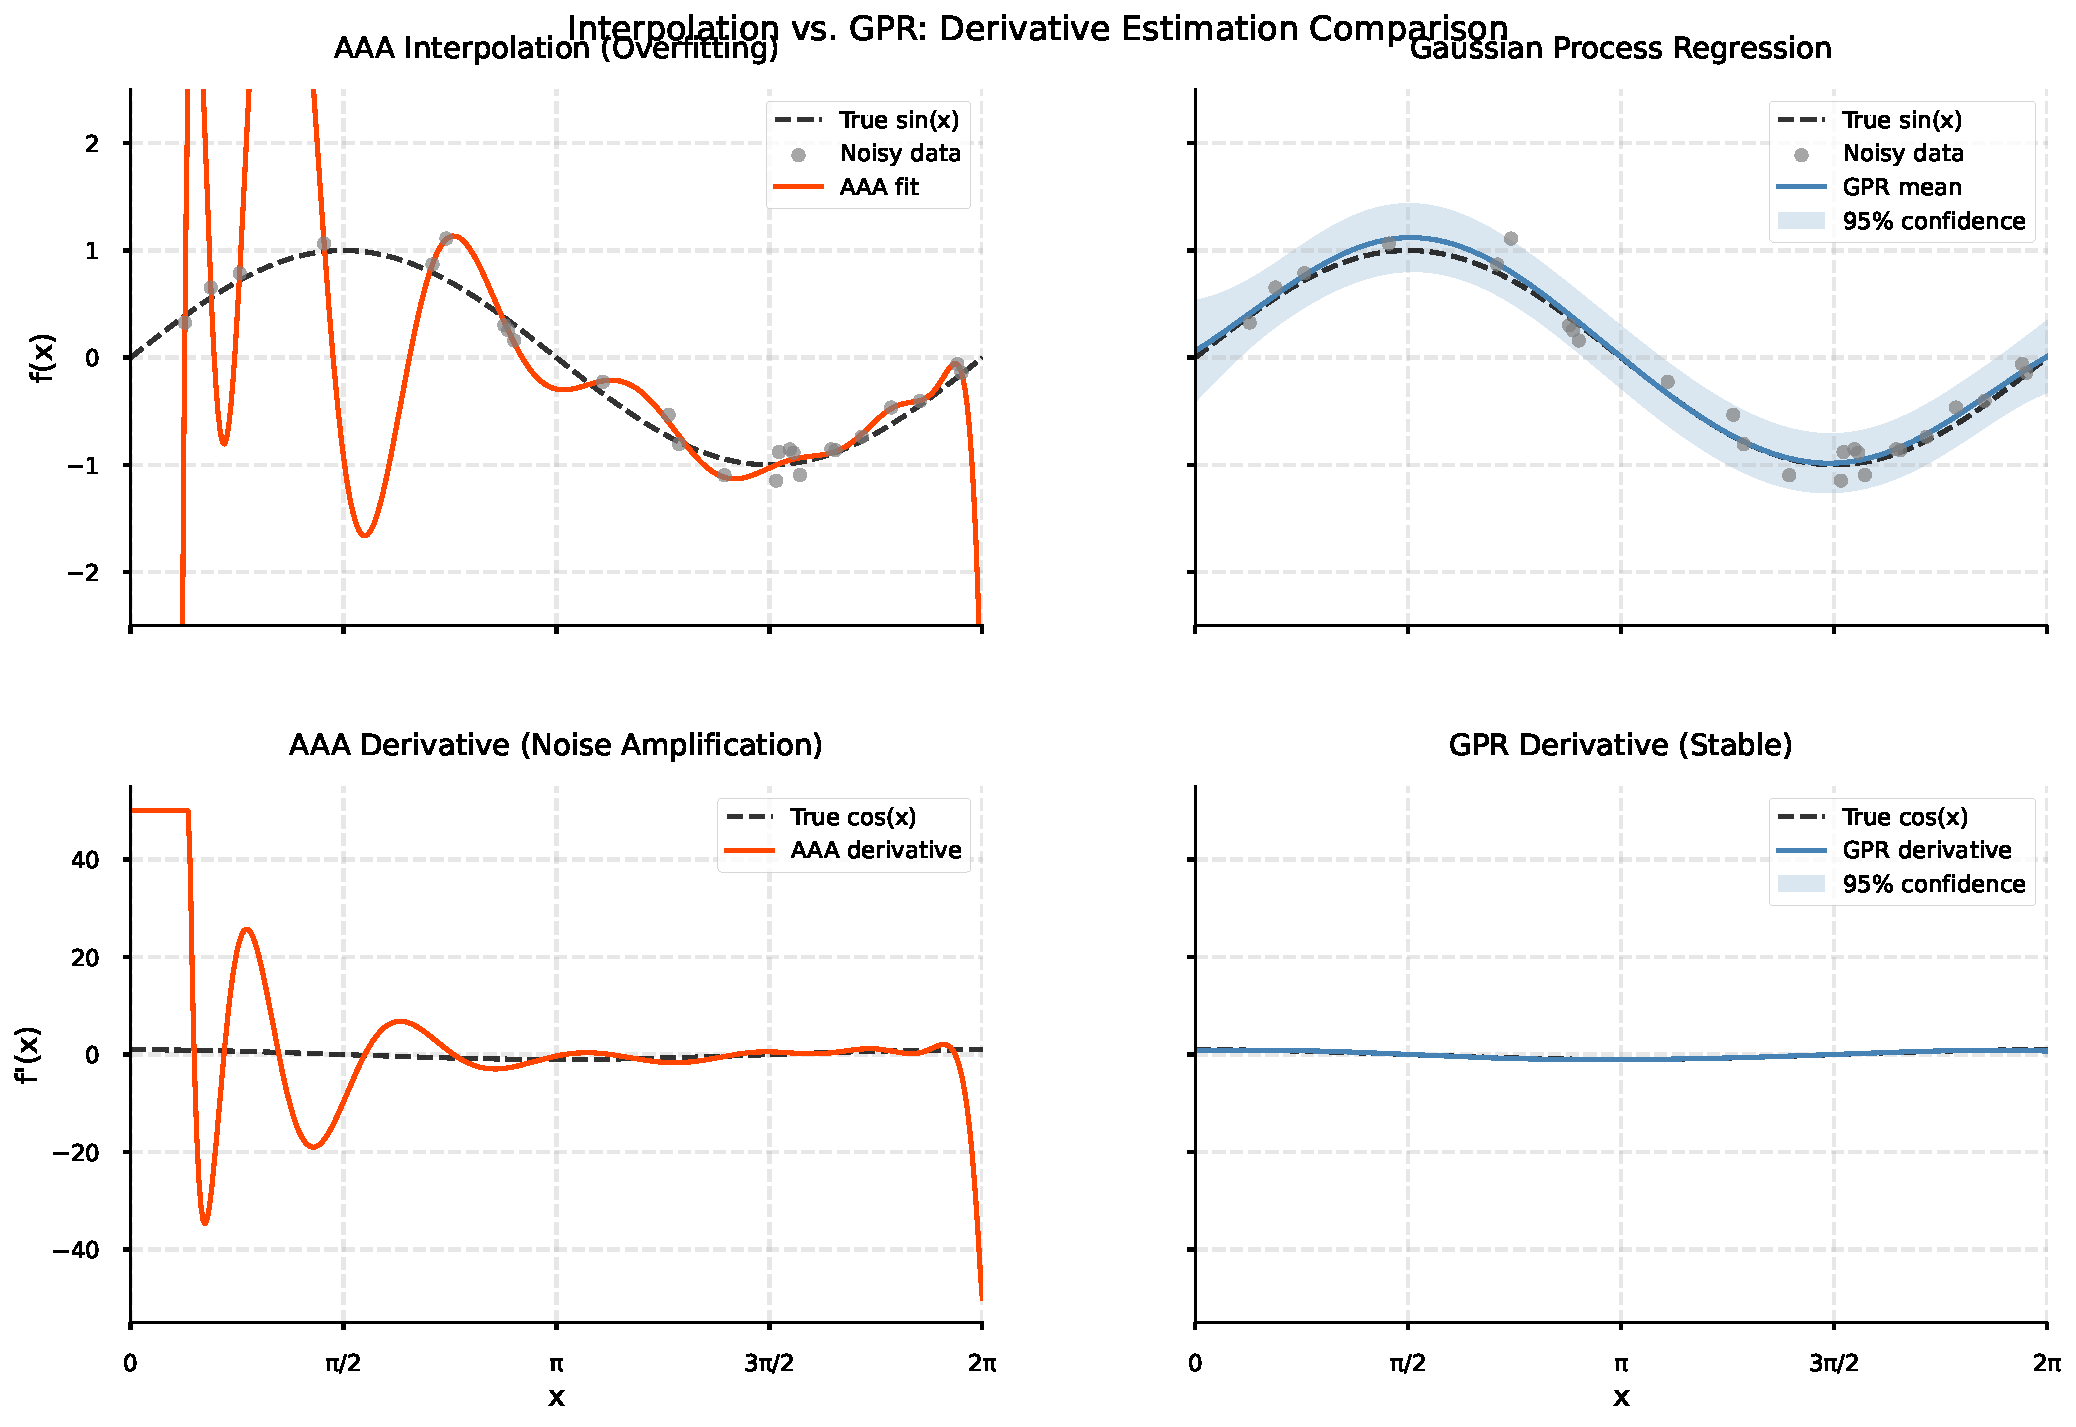
\includegraphics[width=0.9\textwidth]{gpr_vs_aaa_comparison.pdf}
      \end{center}
    \end{column}
    % Right column - GPR approach
    \begin{column}{0.48\textwidth}
      \begin{block}{Solution: Probabilistic Regression}
          \tiny
          We need a method that smooths the data by modeling the underlying function and explicitly accounting for noise. This is a regression problem, not an interpolation problem.
          \begin{itemize}
            \item Function RMSE: 0.059
            \item Derivative RMSE: 0.082
        \end{itemize}
      \end{block}
      \begin{center}
        \textit{Figure included in left panel.}
      \end{center}
    \end{column}
  \end{columns}
\end{frame}

% Slide 6: Our Contribution
\begin{frame}[shrink]{Our Contribution: Gaussian Process Regression}
    \begin{block}{Why Gaussian Process Regression (GPR)?}
    \small
    Instead of fitting a single function, GPR defines a \textit{prior distribution over functions} and updates it to a \textit{posterior distribution} based on the data.
    \begin{itemize}
        \item \textbf{Principled Smoothing:} A smoothness assumption is encoded in the prior via a kernel function (e.g., RBF). This is a natural fit for physical systems.
        \item \textbf{Noise Modeling:} GPR explicitly models measurement noise ($\varepsilon \sim \mathcal{N}(0, \sigma_n^2)$), learning the noise level from the data itself.
        \item \textbf{Analytic Derivatives:} The posterior mean function is a smooth, infinitely differentiable function whose derivatives could be computed analytically.  In practice, we are using automatic differentiation.
        \item \textbf{Noiseless Performance:} In the absence of noise, GPR performance is competitive with high-accuracy interpolation methods, ensuring no significant trade-off.
    \end{itemize}
    \end{block}
    \vspace{1em}
    \begin{alertblock}{Key Idea}
        \centering
        \normalsize
        GPR replaces brittle interpolation with robust Bayesian inference.
    \end{alertblock}
\end{frame}

% Slide 8: Application Benchmark
\begin{frame}[shrink]{Application: End-to-End Parameter Estimation}
    \begin{block}{Benchmark on Nonlinear Systems}
        \centering
        \small
        {\small
\begin{tabular}{@{}l@{\hspace{1pt}}|@{\hspace{2pt}}c@{\hspace{4pt}}c@{\hspace{4pt}}c@{\hspace{1pt}}|@{\hspace{2pt}}c@{\hspace{4pt}}c@{\hspace{4pt}}c@{}}
\toprule
& \multicolumn{3}{c}{\textbf{Lotka-Volterra}} & \multicolumn{3}{c}{\textbf{Van der Pol}} \\
\cmidrule(lr){2-4} \cmidrule(lr){5-7}
\textbf{Noise} & \textbf{GPR} & \textbf{AAA} & \textbf{SciML} & \textbf{GPR} & \textbf{AAA} & \textbf{SciML} \\
\midrule
0.0\% & \textcolor{successgreen}{\textbf{0.0\%}} & 0.0\% & 9.1\% & \textcolor{successgreen}{\textbf{0.0\%}} & 0.0\% & 7.6\% \\
1.0\% & \textcolor{successgreen}{\textbf{4.4\%}} & 29.0\% & 7.7\% & \textcolor{successgreen}{\textbf{0.8\%}} & 7.8\% & 13.5\% \\
5.0\% & \textcolor{successgreen}{\textbf{13.7\%}} & \textcolor{errorred}{$>229\%$} & 4.1\% & \textcolor{successgreen}{\textbf{1.3\%}} & 64.2\% & 6.7\% \\
\bottomrule
\end{tabular}}
        \vspace{0.5em}
        
        \footnotesize
        \textit{Values are Mean Relative Error (MRE) in parameter estimates. `AAA` is the original algebraic method, `SciML` is least-squares direct optimization driven by primarily by Optimization.jl.}
    \end{block}
    
    \begin{columns}[T]
        \begin{column}{0.6\textwidth}
            \begin{alertblock}{Interpretation}
                \footnotesize
                \begin{itemize}
                    \item At zero noise, methods are comparable.
                    \item As noise increases, the AAA-based algebraic method fails catastrophically.
                    \item The GPR-enhanced method remains robust and provides accurate estimates, outperforming the baseline direct optimization.
                \end{itemize}
            \end{alertblock}
        \end{column}
        \begin{column}{0.4\textwidth}
             \begin{block}{Key Advantage}
                \small
                 Our method achieves this accuracy \textbf{without requiring initial guesses} for the parameters.
             \end{block}
        \end{column}
    \end{columns}
\end{frame}

% Slide 9: Conclusion
\begin{frame}[shrink]{Conclusion \& Future Work}
    \begin{columns}[T]
        \begin{column}{0.55\textwidth}
            \begin{block}{Conclusion}
                \begin{itemize}
                    \item We addressed the key bottleneck of the differential-algebraic parameter estimation method by replacing interpolation with Gaussian Process Regression.
                    \item The GPR-enhanced method is robust to realistic noise levels, making it a viable tool for practical applications.
                    \item It preserves the essential advantages of the algebraic approach: it is fully automated and requires no initial parameter guesses.
                \end{itemize}
            \end{block}
        \end{column}
        \begin{column}{0.4\textwidth}
            \begin{block}{Future Work}
                \begin{itemize}
                    \item Propagate GPR derivative uncertainty to parameter estimates.
                    \item Develop ``physics-informed" priors for GPR using the ODE structure.
                    \item Explore sparse GPs to improve computational scaling for large datasets.
                \end{itemize}
            \end{block}
        \end{column}
    \end{columns}
    \vspace{1em}
    \begin{center}
        \small
        \textbf{Software:} \texttt{github.com/orebas/ODEParameterEstimation}
    \end{center}
\end{frame}

% Slide 10: Q&A
\begin{frame}
    \begin{center}
        \huge Thank You
        \vspace{2em}
        
        \Large Questions?
    \end{center}
\end{frame}

% Appendix Slides
\begin{frame}{A1: Benchmark Results - Function Values ($y$)}
    \tiny
    \begin{block}{RMSE for Derivative Order 0}
        \centering
        \begin{tabular}{@{}l|ccc@{}}
\toprule
\textbf{Method} & \textbf{Noise = 0} & \textbf{Noise = 1e-6} & \textbf{Noise = 1e-3} \\
\midrule
AAA\_Julia & {\color{successgreen}$6.2e-7$} & {\color{successgreen}$1.5e-4$} & 0.14 \\
Butterworth\_Python & 0.81 & 0.81 & 0.85 \\
Chebyshev\_Python & 0.12 & 0.12 & 0.16 \\
FiniteDiff\_Python & {\color{successgreen}0.00} & {\color{successgreen}$1.3e-4$} & 0.13 \\
\textbf{GPR\_Julia} & {\color{successgreen}$7.8e-4$} & {\color{successgreen}$7.9e-4$} & {\color{successgreen}0.02} \\
GP\_RBF\_Iso\_Python & {\color{successgreen}$1.3e-3$} & {\color{successgreen}$1.4e-3$} & {\color{successgreen}0.01} \\
KalmanGrad\_Python & 0.19 & 0.15 & 0.22 \\
LOESS\_Julia & {\color{successgreen}0.09} & {\color{successgreen}0.09} & 0.14 \\
SVR\_Python & 0.56 & 0.56 & 0.58 \\
SavitzkyGolay\_Python & {\color{successgreen}0.05} & {\color{successgreen}0.05} & {\color{successgreen}0.09} \\
TVDiff\_Julia & {\color{successgreen}$2.5e-14$} & {\color{successgreen}$1.3e-4$} & 0.13 \\
\bottomrule
\end{tabular}

    \end{block}
    \begin{alertblock}{Interpretation}
        For function value estimation (order 0), most methods perform reasonably well. Interpolation methods like AAA are extremely accurate on noise-free data, but GPR is more stable as noise increases.
    \end{alertblock}
\end{frame}

\begin{frame}{A2: Benchmark Results - 3rd Derivative ($y'''$)}
    \tiny
    \begin{block}{RMSE for Derivative Order 3}
        \centering
        \begin{tabular}{@{}l|ccc@{}}
\toprule
\textbf{Method} & \textbf{Noise = 0} & \textbf{Noise = 1e-6} & \textbf{Noise = 1e-3} \\
\midrule
AAA\_Julia & {\color{successgreen}0.53} & {\color{errorred}$2.2e5$} & {\color{errorred}$1.3e9$} \\
Butterworth\_Python & 28.90 & 28.90 & 28.90 \\
Chebyshev\_Python & 60.56 & $8.9e2$ & {\color{errorred}$1.8e5$} \\
FiniteDiff\_Python & 45.19 & {\color{errorred}$1.9e4$} & {\color{errorred}$2.0e7$} \\
\textbf{GPR\_Julia} & {\color{successgreen}9.44} & {\color{successgreen}9.45} & 19.93 \\
GP\_RBF\_Iso\_Python & 16.79 & 16.78 & 13.84 \\
KalmanGrad\_Python & 37.80 & 27.62 & 34.38 \\
LOESS\_Julia & {\color{errorred}$8.1e4$} & {\color{errorred}$5.2e8$} & {\color{errorred}$1.1e4$} \\
SVR\_Python & 28.58 & 28.58 & 28.58 \\
SavitzkyGolay\_Python & 22.97 & {\color{errorred}$1.8e4$} & {\color{errorred}$2.2e7$} \\
TVDiff\_Julia & $1.5e2$ & {\color{errorred}$3.1e3$} & {\color{errorred}$6.5e3$} \\
\bottomrule
\end{tabular}

    \end{block}
    \begin{alertblock}{Interpretation}
        For 3rd order derivatives, the difference is stark. GPR is the only tested method that remains robust and accurate across all noise levels. Other methods either fail catastrophically or, like SVR, have large but stable errors.
    \end{alertblock}
\end{frame}

\end{document}
